\section{量子カオスとしてのブラックホール\label{sec:gravity}}
この節では主にSYK模型の重力双対であるJackiw--Teitelboim(JT)ブラックホールの量子カオスの性質を述べる
\footnote{この節の内容は\cite{polchinski_chaos}及び\cite{stanford_chaos}による。}。
特に\eqref{eq:spectral_form_factor}式で定義されるスペクトラル形状因子の
slopeとrampを与えるような時空の計量はどのようなものかという事を議論する。
ここで注意するべきは、JTディラトン重力はSYK模型のようなdisorderを持つ理論ではないため、
$\average{ZZ^*}$のような期待値計算ではなく$ZZ^*$そのものの計算となるという事である
\footnote{SYK模型においても期待値を外して$ZZ^*$を計算する事はもちろん可能である。
この時にrampやplateauを数値解析によりプロットすると大きい揺らぎを目視する事ができる。
一方でこの節で計算するJT重力の$ZZ^*$には、disorder averageを取っていないにも関わらず、
揺らぎが存在しない。この点は今後の課題の1つである。詳しくは第\ref{sec:conclusion}節を参照。}。

第\ref{sec:fourpointfunc}節で論じたように、SYK模型は低エネルギーでシュワルツ理論となるため、
前節で論じた鞍点もシュワルツ理論によって記述できる。
一般にシュワルツ理論はJTディラトン重力理論と等価である事が知られており、従って前節の$G$と$\Sigma$の配位は
AdS/CFT対応におけるバルク側のJTディラトン重力として理解できる。
ただし$G$と$\Sigma$の配位というのは重力側では計量の配位として翻訳されるべきものである。
従ってここでの問題はSYK模型で議論した鞍点は重力側ではどのような時空の幾何学に対応するかという事である。

前節と同様にここでも2つのレプリカが現れ、それぞれL系とR系と名付ける事にすると、
前節の$G$と$\Sigma$の配位に全く対応した解が現れる。
即ち、L系とR系に相関がないような解がslopeを与え、また両レプリカ系に相関が存在し、
かつ各々が独立に持っていた時間並進対称性が自発的に破れるような解はrampとして寄与する。
ちなみに一般相対性理論で計量のアイソメトリーを意味するKillingベクトル場と対応して、
JTディラトン重力理論の計量が時間方向の並進でアイソメトリーを持つ事から、
この時間座標をKilling時間と呼ぶ事にする。

L系とR系はここではdiskのトポロジーを持つブラックホールに対応し、特にrampを与えるような解は
この2つのブラックホールをつなぐようなワームホールと呼ばれるものとなる。
以下では上述した事の詳細を述べる。

\subsection{JTディラトン重力}
まず最初にJTディラトン重力について簡単に紹介する。
作用は次式で与えられる:
\begin{align}
	S_{JT} = -\frac{\phi_0}{2}\left[\int \sqrt{g}R + 2\int_{bdy}\sqrt{h}K \right]
			-\frac{1}{2}\left[
				\int \sqrt{g}\phi(R+2) + 2\phi_b\int_{bdy}\sqrt{h}K
			\right].
\end{align}
この理論は高次元のAdS空間を2次元にコンパクト化する事で得られる。
ディラトン$\phi$はその際のコンパクト化半径に対応する。
$\phi$について変分する事で得られる運動方程式はリッチスカラーに関する方程式であり、$R = -2$となる。
これにより2次元においては局所的な時空の幾何が$\mathrm{AdS}_2$の一部分として固定される。
問題はどの部分が$Z(\beta + iT)Z(\beta - iT)$の計算に関わるかである。

\subsection{slopeおよびramp: 直感的な説明}
1つの選択肢は互いに離れている2つの幾何であり、それぞれは逆温度$\beta + iT$および$\beta - iT$を持つ
ブラックホールに対応し、diskのトポロジーを持つ。
これはSYK模型の話における$G_{LR} = 0$の解に対応し、slopeを構築する。
従ってラージ$T$でゼロに落ちていく。

しかし、L系とR系が互いに相関するような別の選択肢も存在する。
具体的には、図\ref{fig:double_cone}の右側の図のようにL系とR系のブラックホールを
円錐で接するようにしたものである。この解を2重円錐と呼ぶ事にする。
まずこの解について直感的に説明する。

\begin{figure}[ht]
	\centering
	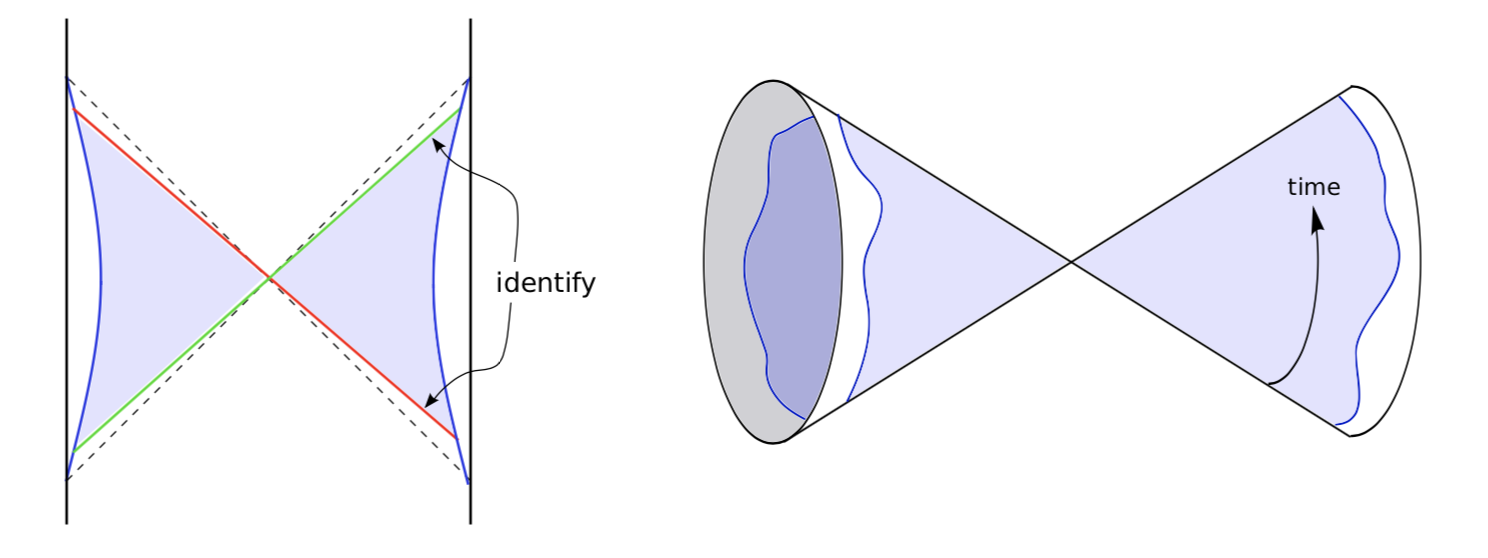
\includegraphics[width=10cm]{figures/double_cone}
	\caption{
	2重円錐。左図では同一視化の2つの表面(矢印で示した赤と緑の線)を示した。
	青の曲線は境界を表す。
	右図では左図を同一視する表面で折りたたんだ2重円錐を表した。
	また左図で境界を表していた青い曲線は右図ではより歪んだ曲線としている。
	これは境界の重力子の自由度を考慮している。
	この図は\cite{polchinski_chaos}より引用した。}
	\label{fig:double_cone}
\end{figure}

JT重力の最も単純なLorentzian解は次式のリンドラー座標に対応する:
\begin{align}
	ds^2 = -\sinh^2(\rho)d\tilde{t}^2 + d\rho^2,\hspace{20pt}
	\phi = \phi_h\cosh(\rho).
\end{align}
この座標は$\tilde{t}$の並進対称性を持つ。
大雑把に言えば、これに$\tilde{t}\sim\tilde{t}+\tilde{T}$という同一視を加えた幾何を求めたいのである。
言い換えればリンドラー領域をあるブーストで同一視する。
このブーストはR側の境界では時間を進める方向への並進であり、一方でL側の境界では時間を戻す方向への並進
であるため、この同一視は$Z(iT)Z(-iT)$への適切な周期性を定める。
これは図\ref{fig:double_cone}のような閉じた時間的曲線を持つ2重円錐として可視化でき、
2つの円錐の頂点は$\rho = 0$で接する。
この$\rho = 0$という点は$\tilde{t}\sim\tilde{t}+\tilde{T}$という同一視の固定点である。
また2重円錐解には2つのパラメータが存在し、1つ目は$\tilde{T}$と$T$の関係から与えられる。
これは$\beta_{aux}$に対応するものである事を後に見る。
もう1つ目はL側とR側の両境界の時間座標の原点をどこに設置するかという自由度に起因する。
同一視を施された幾何の持つ時間並進対称性により、L系とR系にの時間座標の原点に対する並進を同時に行っても
何も起こらないが、相対的な並進ならば意味を持つ。
つまり、SYK模型での解のように、2重円錐による解はL系とR系がそれぞれ独立に持つ時間並進対称性を
自発的に破り、$T$に比例する体積を持つゼロモード$\Delta t$が誕生する。
これがrampの説明の候補となる。

\subsection{slopeおよびramp: 系統的な理解}
ここでは前節のslopeやrampの議論を、より系統的なものにする。


\pagebreak